%!TEX root = ../main.tex
%%%%%%%%%%%%%%%%%%%%%%%%%%%%%%%%%%
% Links:
%
% Difficulty:
% Companies: 
%%%%%%%%%%%%%%%%%%%%%%%%%%%%%%%%%%


%\begin{figure}
%	\centering
%	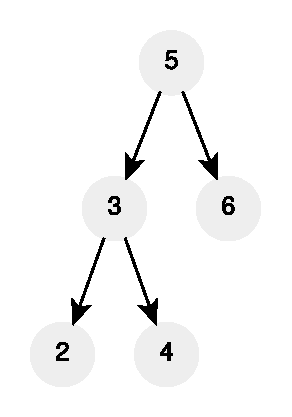
\includegraphics[width=\textwidth]{sources/smallest_range/images/example1}
%	\caption[Sample short cpation]{Sample Caption}.
%	\label{fig:smallest_range:example1}
%\end{figure}

\chapter{Smallest Range \RN{1} and \RN{2}}
\label{ch:smallest_range}
\section*{Introduction}

\section{Problem statement}
\begin{exercise}
\label{example:smallest_range:exercice1}
Write a function that given given an array of integers $I$ and an integer $K$ 
returns the smallest possible difference between the smallest and largest value in $I$
after you have added to each of the elements $-K \leq p \leq K$.

	%example1
	\begin{example}
		\label{example:smallest_range:example1}
		\hfill \\
		Given $I = \{3,5,1,7,8\}$ and $K=4$ the function returns $0$. You can modify add to $I$ the followings values
		$\{1,-1,3,-3,-4\}$. The modified array finally becomes: $I'=\{4,4,4,4,4\}$. 
		
	\end{example}

	%example2
	\begin{example}
		\label{example:smallest_range:example2}
		\hfill \\
		Given $I = \{1,9,4\}$ and $K=2$ the function returns $4$.
	\end{example}

\end{exercise}

\section{Clarification Questions}

\begin{QandA}
	\item Can you add $p$ multiple times to an element of $I$?
	\begin{answered}
		\textit{No, you can only add $p$ once to each element of $I$.}
	\end{answered}	
\end{QandA}

\section{Discussion}
\label{smallest_range:sec:discussion}


\subsection{Brute-force}
\label{smallest_range:sec:bruteforce}

\begin{minipage}{\linewidth}
	\lstinputlisting[language=c++, caption={Sample Caption},label=list:smallest_range]{sources/smallest_range/smallest_range_solution1.cpp}
\end{minipage}


\section{Common Variations}
\subsection{Smallest range \RN{2} }
This variant is almost identical to the main problem of this chapter (Exercice \ref{}) except that this time
we are only allowed to add either $-K$ or $+K$ to each and every element of the input array $I$. As we shall see, this complicates things quite a bit,
but, nevertheless, the core solution strategy  remains the same. 

\begin{exercise}
	\label{example:smallest_range:variation1:exercice1}
	Write a function that given given an array of integers $I$ and an integer $K$ 
	returns the smallest possible difference between the smallest and largest value in $I$
	after you have added to each of the elements either $-K$ or $K$.
	
		%example1
		\begin{example}
			\label{example:smallest_range:variation1:example1}
			\hfill \\
			Given $I = \{3,5,1,7,8\}$ and $K=4$ the function returns $xxx$. You can modify add to $I$ the followings values
			$\{xxxxx\}$. The modified array finally becomes: $I'=\{xxxxx\}$. 
			
		\end{example}
	
		%example2
		\begin{example}
			\label{example:smallest_range:variation1:example2}
			\hfill \\
			Given $I = \{1,9,4\}$ and $K=2$ the function returns $xxxxx$.
		\end{example}
	
	\end{exercise}
